% !TEX TS-program = pdflatex
% !TEX encoding = UTF-8 Unicode

\documentclass[a4paper, titlepage=false, parskip=full-, 10pt]{scrartcl}

\usepackage[utf8]{inputenc}
\usepackage[T1]{fontenc}
\usepackage[english, ngerman]{babel}
\usepackage{babelbib}
\usepackage{hyperref}
\usepackage{listings}
\usepackage{framed}
\usepackage{color}
\usepackage{graphicx}
\usepackage[normalem]{ulem}
\usepackage{cancel}
\usepackage{array}
\usepackage{amsmath}
\usepackage{amssymb}
\usepackage{amsthm}
\usepackage{algorithm}
\usepackage{algorithmic}
\usepackage{geometry}
\usepackage{subfigure}
\geometry{a4paper, top=20mm, left=35mm, right=25mm, bottom=40mm}

\newcounter{tasknbr}
\setcounter{tasknbr}{1}
\newenvironment{task}[1]{{\bf Aufgabe \arabic {tasknbr}\stepcounter{tasknbr}} (#1):\begin{enumerate}}{\end{enumerate}}
\newcommand{\subtask}[1]{\item[#1)]}

% Listings -----------------------------------------------------------------------------
\definecolor{red}{rgb}{.8,.1,.2}
\definecolor{blue}{rgb}{.2,.3,.7}
\definecolor{lightyellow}{rgb}{1.,1.,.97}
\definecolor{gray}{rgb}{.7,.7,.7}
\definecolor{darkgreen}{rgb}{0,.5,.1}
\definecolor{darkyellow}{rgb}{1.,.7,.3}
\lstloadlanguages{C++,[Objective]C,Java}
\lstset{
escapeinside={§§}{§§},
basicstyle=\ttfamily\footnotesize\mdseries,
columns=fullflexible,
keywordstyle=\bfseries\color{blue},
commentstyle=\color{darkgreen},      
stringstyle=\color{red},
numbers=left,
numberstyle=\ttfamily\scriptsize\color{gray},
breaklines=true,
showstringspaces=false,
tabsize=4,
captionpos=b,
float=htb,
frame=tb,
frameshape={RYR}{y}{y}{RYR},
rulecolor=\color{black},
xleftmargin=15pt,
xrightmargin=4pt,
aboveskip=\bigskipamount,
belowskip=\bigskipamount,
backgroundcolor=\color{lightyellow},
extendedchars=true,
belowcaptionskip=15pt}

%% Enter current values here: %%
\newcommand{\lecture}{Robotik WS15/16}
\newcommand{\tutor}{}
\newcommand{\assignmentnbr}{7}
\newcommand{\students}{Julius Auer, Thomas Tegethoff}
%%-------------------------------------%%

\begin{document}  
{\small \textsl{\lecture \hfill \tutor}}
\hrule
\begin{center}
\textbf{Übungsblatt \assignmentnbr}\\
[\bigskipamount]
{\small \students}
\end{center}
\hrule

\begin{task}{Control}\item[]
Wir betrachten - wie vorgeschlagen - als Fehler nicht den absoluten Positions-Fehler, sondern den Winkel zur Wunschtrajektorie. Auf allen Plots sieht man:

\begin{itemize}
\item die aktuelle y-Position (blau)
\item die Abweichung des Yaws im World-Frame vom Wunsch-Winkel ($=$Fehler) (rot)
\item den Regelausgang (cyan)
\end{itemize}

Das Auto startet immer bei $y=3$ und versucht $y=-0.5$ (Mitte der rechten Spur) zu erreichen. Die Vorausschaustrecke $a$ zur Berechnung des Wunschwinkels ist stets $a=4m$ - für einen größeren Wert arbeiten einfachste P-Regler schon perfekt und es ist seht schwer das System zum oszillieren zu bringen. Ebenso willkürlich gewählt sind die Konstanten für Beschleunigung und Lenkbeschleunigung. Bei schlecht gewählten Konstanten neigt das Auto dazu Unfälle zu verursachen (üblicherweise in Form von Überschlägen). Es wäre nett gewesen, wenn wir hierfür eine Vorgabe gehabt hätten - überhaupt ein funktionierendes System zu konstruieren war mal wieder etwas kniffelig ;)

\subtask{a}
Grundsätzlich ist ein großer P-Anteil $K_p$ erstrebenswert, um sich rasch der Wunschtrajektorie anzunähern. Der - experimentell ermittelt - größte Wert bei dem das Auto keinen Unfall baut (aufgrund zu starker Lenkbewegungen) ist $K_p=0.1$, was das in Abbildung \ref{fig:1} gezeigt Ergebnis liefert.
 
 Arbeitet man zusätzlich mit einem D-Anteil, kann der P-Anteil ggf. größer gewählt werden: gesucht wurde deshalb für $K_p=0.2$ ein D-Anteil $K_d$ der so klein wie möglich ist, aber das Übersteuern verhindern. Für $K_p=0.1,K_d=0.3$ ergibt sich das in Abbildung \ref{fig:2} dargestellte Bild.
 
 \newpage
\subtask{b}
Das System oszilliert bei $K_{p_k}=0.05$. Abbildung \ref{fig:3} zeigt ferner, dass die Periodenlänge $t$ in etwa $t=4$ ist. Nach Ziegler/Nichols ergeben sich somit die Regelanteile zu:

\begin{align*}
K_p&=0.6\cdot K_{p_k}&=0.03\\
K_i&=\frac{2\cdot K_p}{t}&=0.015\\
K_d&=0.12\cdot K_p\cdot t&=0.0144
\end{align*}

Wobei nirgendwo erwähnt wird (oder??) wie groß das ''Gedächtnis'' sein soll, was aber einen signifikanten Einfluss auf die Größe des I-Anteils hat. Wählt man die Gedächtnis-Größe zu groß, gibt es wieder Überschläge.\\
Mit diesen Anteilen erhält man die in Abbildung \ref{fig:4} gezeigte Situation.

Ergebnisse:
\begin{itemize}
\item Der P-Regler stabilisiert sich nach ca. 12s ganz OK
\item Der PD-Regler stabilisiert sich nach ca. 10s super
\item Der PID-Regler stabilisiert sich nicht wirklich (oszilliert schwach), ist aber für diese Situation auch ungeeignet (keine Störgrößen vorhanden)
\end{itemize}

\newpage
\begin{figure}[!htpb]
\begin{center}
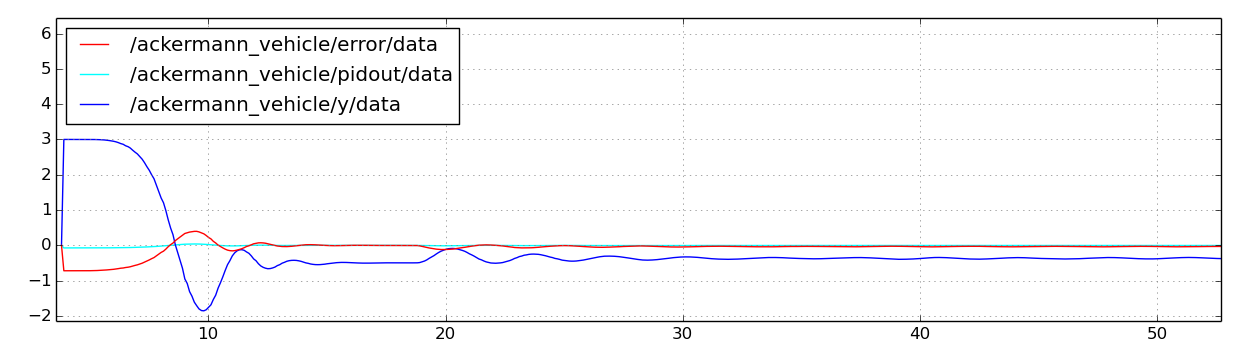
\includegraphics[width=0.9\linewidth]{capture1}
\end{center}
\caption{P-Regler}
\label{fig:1}
\end{figure}
\begin{figure}[!htpb]
\begin{center}
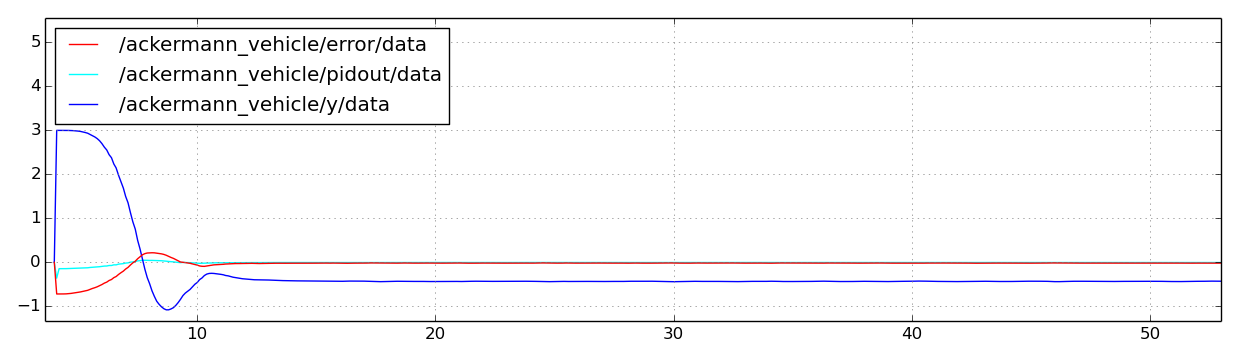
\includegraphics[width=0.9\linewidth]{capture2}
\end{center}
\caption{PD-Regler}
\label{fig:2}
\end{figure}
\begin{figure}[!htpb]
\begin{center}
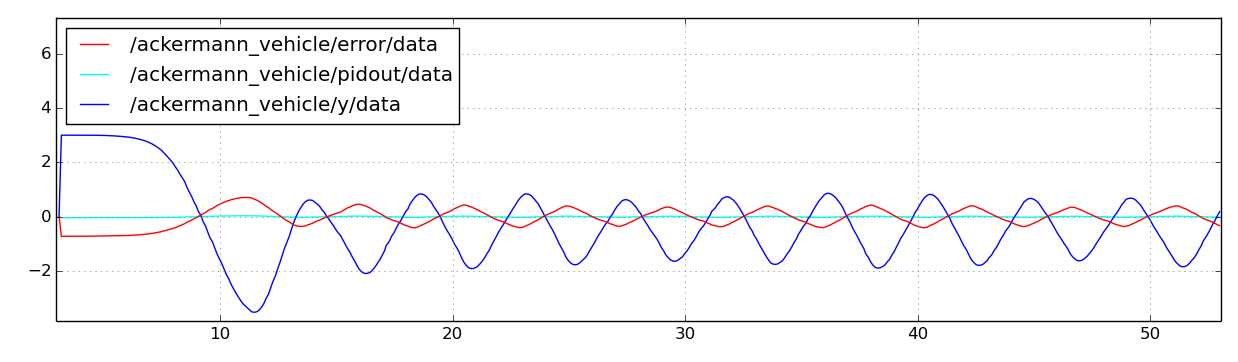
\includegraphics[width=0.9\linewidth]{capture3}
\end{center}
\caption{P-Regler (oszillierend)}
\label{fig:3}
\end{figure}
\begin{figure}[!htpb]
\begin{center}
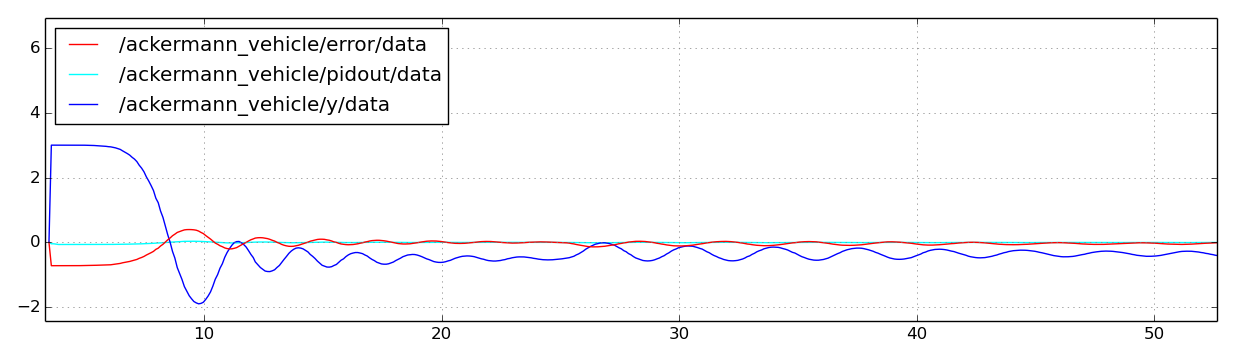
\includegraphics[width=0.9\linewidth]{capture4}
\end{center}
\caption{PID-Regler nach Ziegler/Nichols}
\label{fig:4}
\end{figure}
\end{task}
\end{document}